\chapter{System Architecture}
\label{chap:system-architecture}

This chapter describes the architecture of the True Demand KGQA system. The system is designed as a controlled natural-language interface over a survey-grounded knowledge graph, where the main challenge is not only to generate SPARQL, but to select, validate, and execute the interpretation that best matches the user's intent. The architecture therefore combines deterministic graph-supported routing, LLM-based candidate generation, schema and semantic validation, ML-based query selection, confidence-aware routing, and a user interface that exposes clarification and evidence when needed.

The central design principle is that the LLM should not be treated as the only reasoning component. Instead, the LLM is one component inside a broader decision pipeline. Direct graph-supported queries are answered without using the LLM, ambiguous cases are routed through candidate generation and ranking, and high-uncertainty cases are not forced into an automatic answer. This structure is important for three reasons:

\begin{itemize}
    \item \textbf{Reliability}: a syntactically valid SPARQL query can still answer the wrong business question, so query selection must be validated and ranked.
    \item \textbf{Cost}: LLM calls are expensive in the enterprise environment, so simple graph-supported questions should be answered deterministically where possible.
    \item \textbf{Usability}: when a question is genuinely ambiguous, the user should see clear alternatives in natural language rather than raw SPARQL.
\end{itemize}

Figure~\ref{fig:system-architecture-pipeline} shows the final architecture at a high level. The user interacts with the Streamlit application. The application first attempts cheap request routing and direct capability matching. If no exact graph-supported route is found, the system uses the LLM to generate candidate SPARQL queries. These candidates are validated, featurized, ranked, and routed through a confidence policy before the selected query is executed against the True Demand graph.

\begin{figure}[ht]
\centering
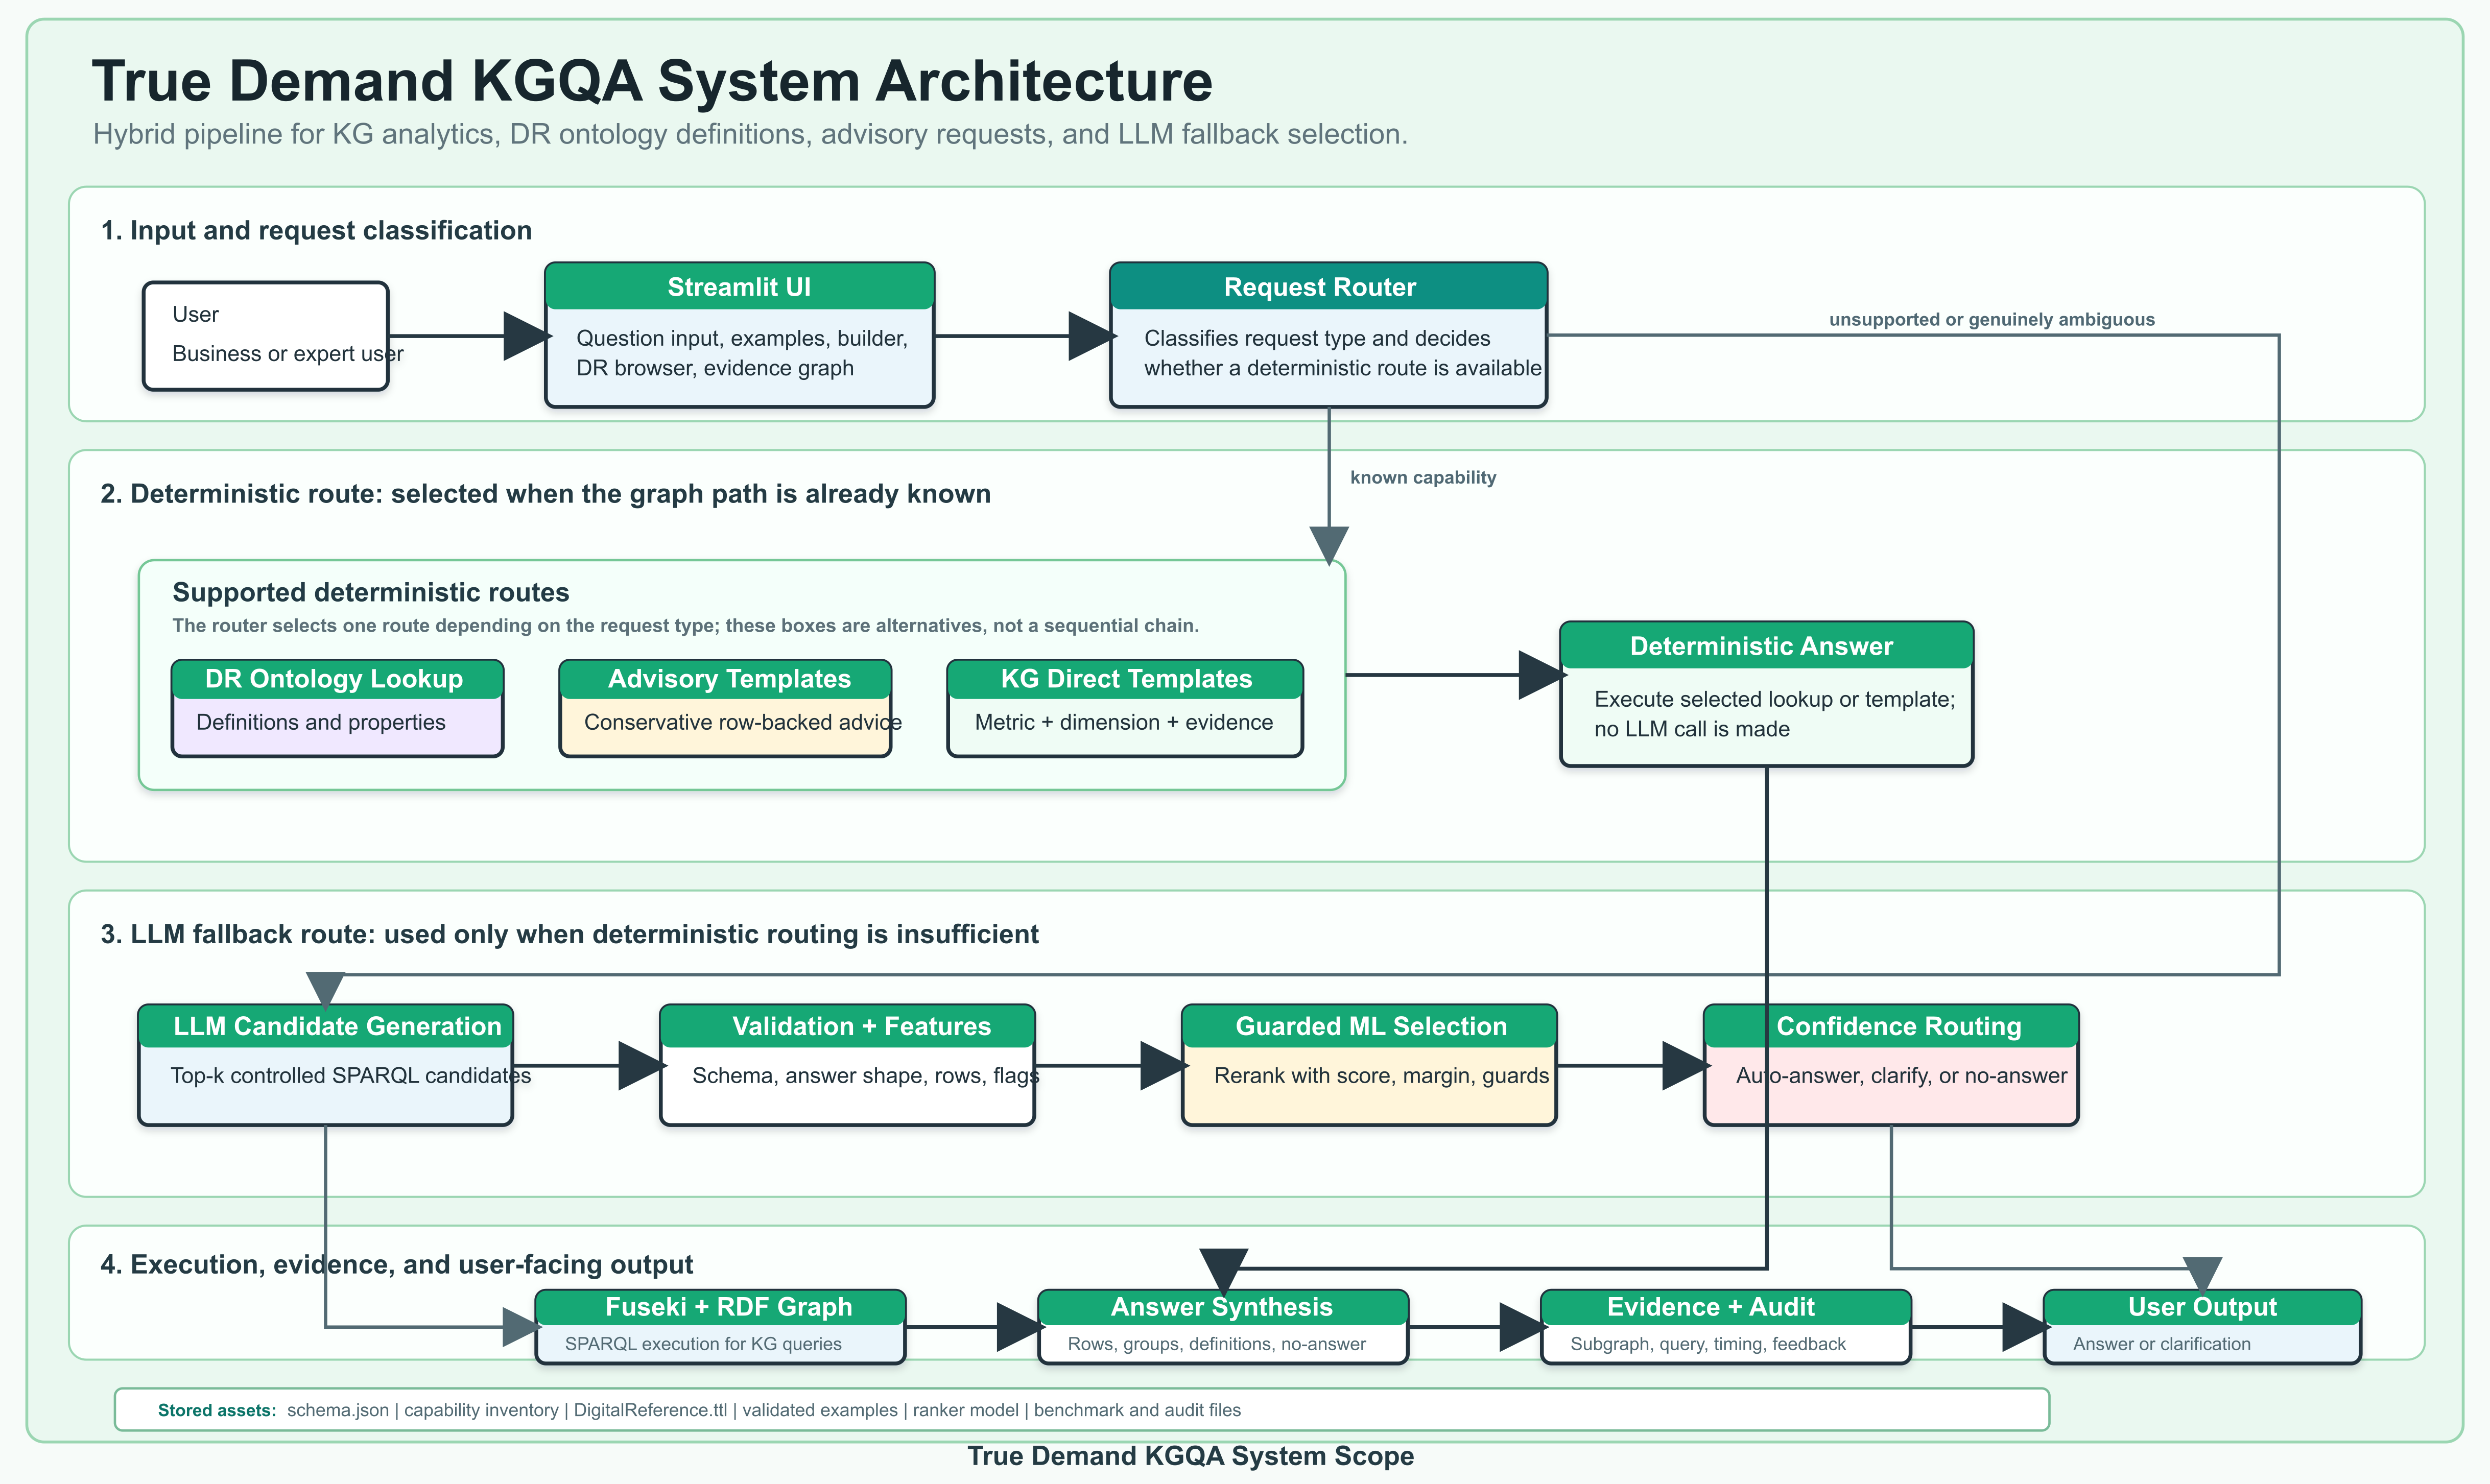
\includegraphics[width=0.98\textwidth]{docs/figures/system_architecture_pipeline.png}
\caption{Overall architecture of the True Demand KGQA system.}
\label{fig:system-architecture-pipeline}
\end{figure}

\section{Overall Pipeline}
\label{sec:overall-pipeline}

The system follows a staged pipeline. Each stage either reduces ambiguity, validates an interpretation, or decides whether the system should answer automatically. This staged design is different from a simple LLM-to-SPARQL setup, where a single generated query is executed immediately. In the proposed system, execution is only the final step after routing, generation, validation, selection, and confidence assessment.

At runtime, the system receives a natural-language question from the user. The question is first passed through lightweight routing components. These components check whether the request is a graph question, a definition-style request, an unsupported request, or a direct graph-supported analytical query. If the question matches a known capability pattern, such as current demand by region or vehicle sales by month, the system can generate the SPARQL query deterministically and execute it without calling the LLM.

If direct routing is not possible, the system moves to the LLM candidate-generation path. The LLM is provided with a controlled schema context and asked to generate multiple SPARQL candidates rather than a single answer. This is important because many user questions can be interpreted in several plausible ways. The candidate set is then processed by validation and feature-extraction components. These components extract syntax validity, schema consistency, query-plan information, answer shape, selected variables, aggregation type, grouping variables, and domain-specific contract features.

The ranking stage uses these features to score the candidates. In the final system, the main ML selector is a lightweight NP/TF-IDF logistic reranker trained on grouped candidate sets. The model is used with guard conditions rather than as an unconditional override: a switch is only accepted when score, margin, and rank constraints are satisfied. This prevents unstable low-confidence switches from reducing reliability.

Finally, the confidence and ambiguity routing layer decides whether the system should answer automatically, ask the user for clarification, or expose alternative interpretations. The selected query is executed through Fuseki when a SPARQL endpoint is available, with an RDFLib fallback for local execution. The answer synthesis module then converts the result rows into natural language and displays the associated graph evidence in the UI.

\begin{table}[ht]
\centering
\caption{Main runtime stages in the True Demand KGQA architecture.}
\label{tab:runtime-stages}
\begin{tabular}{p{3.2cm}p{5.2cm}p{5.2cm}}
\hline
\textbf{Stage} & \textbf{Purpose} & \textbf{Main output} \\
\hline
Request routing & Determine whether the request is a KG query, definition request, unsupported request, or direct capability query & Route label and optional direct query \\
Capability resolution & Detect graph-supported metric, dimension, and aggregation patterns & Capability report and direct template match \\
LLM candidate generation & Generate multiple SPARQL interpretations when direct routing is insufficient & Candidate query set \\
Validation and feature extraction & Check syntax, schema consistency, semantic coverage, and query shape & Candidate feature vectors and safety flags \\
ML-based selection & Rank candidates and apply guarded selection rules & Selected candidate and selection scores \\
Confidence routing & Decide whether to answer, clarify, or abstain from forced selection & Auto-answer or clarification decision \\
Execution & Run the selected query against the graph & Rows, errors, and evidence paths \\
Answer synthesis & Convert rows into a concise natural-language answer & User-facing answer and evidence summary \\
\hline
\end{tabular}
\end{table}

Listing~\ref{lst:overall-runtime-pipeline} summarizes the pipeline in pseudocode. The actual implementation is distributed across \texttt{app.py}, \texttt{pipeline/qa.py}, \texttt{kg/capabilities.py}, \texttt{ranking/}, \texttt{validation/}, and \texttt{llm/answer\_synthesis.py}.

\begin{lstlisting}[caption={Simplified runtime pipeline for one user question.}, label={lst:overall-runtime-pipeline}]
question = read_user_question()

route = route_request(question)
if route is not graph_question:
    return route_specific_response(route)

capability = resolve_graph_capability(question)
if capability has one exact graph-supported query:
    query = capability.direct_query
    rows = execute(query)
    return synthesize_answer(question, query, rows)

candidates = generate_llm_candidates(question, schema_context)
features = extract_validation_and_query_features(candidates)
ranked = rank_candidates_with_ml_or_schema(features)

decision = confidence_route(ranked)
if decision == auto_answer:
    rows = execute(ranked.top.query)
    return synthesize_answer(question, ranked.top.query, rows)

if decision == clarify:
    return show_top_interpretations(ranked.top_k)
\end{lstlisting}

The important point is that the architecture separates \emph{generation} from \emph{selection}. The LLM is responsible for producing candidate interpretations. The system is responsible for deciding whether any of these interpretations should be trusted.

\section{Direct Graph-Supported Routing}
\label{sec:direct-graph-supported-routing}

Direct graph-supported routing is the first major control layer. Its purpose is to answer frequent, unambiguous, graph-supported questions without using the LLM. This reduces cost and latency, and it also avoids unnecessary ambiguity when the graph already contains a known analytical pattern.

A direct route is not a keyword shortcut alone. It is based on a capability definition: a metric, a dimension, an aggregation intent, and a SPARQL template that is known to return rows over the current graph. For example, a question such as ``Show total current demand from OEM customers by region'' can be mapped to a deterministic regional-demand query if the system detects the current-demand capability, the OEM scope, and the region dimension. Similarly, vehicle sales by month, shortage counts by status, and autonomous-driving averages by vehicle type can be expressed as known graph-supported templates.

The capability registry is implemented in \texttt{kg/capabilities.py}. Each capability contains aliases, required core graph terms, supported dimensions, aggregation options, and in some cases direct query templates. This registry is used by the UI autocomplete, direct routing, clarification filtering, and efficiency evaluation scripts.

\begin{figure}[ht]
\centering
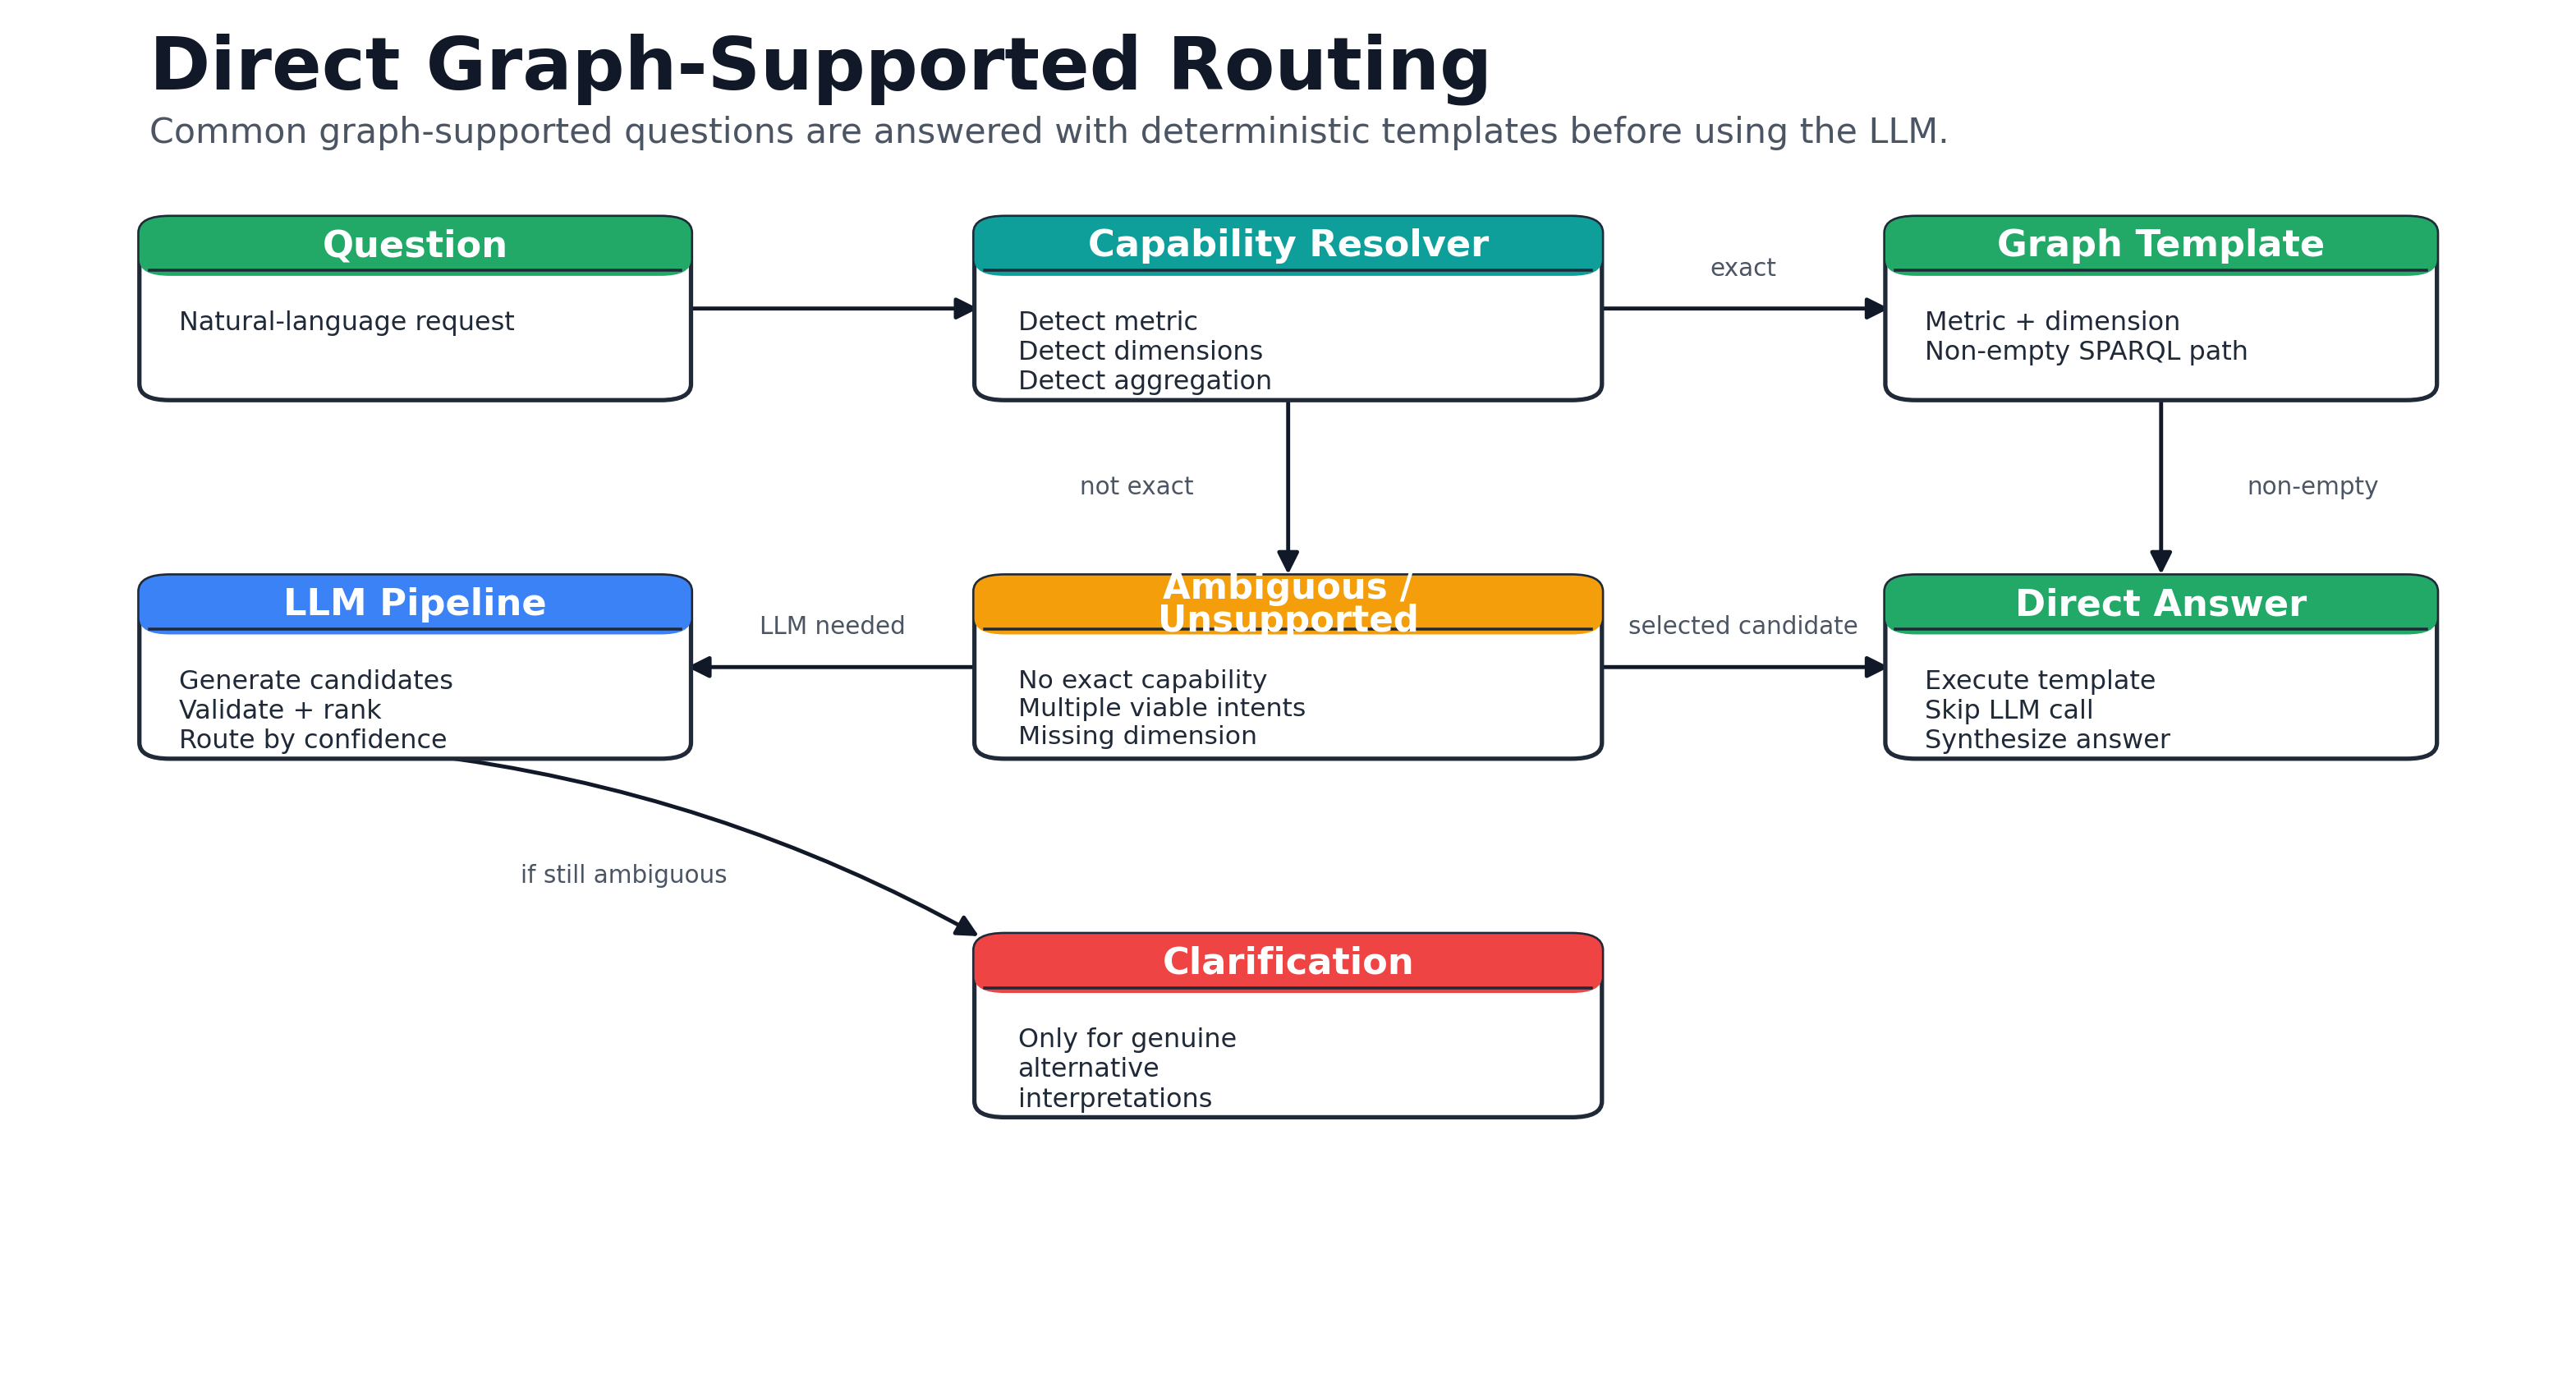
\includegraphics[width=0.92\textwidth]{docs/figures/direct_graph_supported_routing.png}
\caption{Direct graph-supported routing before LLM candidate generation.}
\label{fig:direct-graph-routing}
\end{figure}

The direct routing layer is intentionally conservative. It should only return a direct query when the user's request is specific enough. The system should not convert a broad phrase such as ``demand by region'' into a specific query if several demand capabilities remain plausible, such as current demand, future demand, OEM demand, or semiconductor demand. In such cases, clarification is more appropriate.

\begin{table}[ht]
\centering
\caption{Examples of direct graph-supported route families.}
\label{tab:direct-route-families}
\begin{tabular}{p{3.4cm}p{5.5cm}p{4.8cm}}
\hline
\textbf{Family} & \textbf{Direct patterns} & \textbf{Why it can be direct} \\
\hline
Current / regional demand & Total or average demand by region, survey group, or vehicle type & Metric and grouping dimensions are explicit and graph-supported \\
Future demand & Future demand change by region, quarter, vehicle type, or technology category & Capability has predefined analytical paths \\
Vehicle sales & Vehicle-sales units by month, year, or vehicle type & Large observation table with stable time dimensions \\
Shortage & Count companies by shortage status or survey group & Count shape and target class are clear \\
Autonomous driving & Average development percentage by vehicle type, SAE level, year, or survey group & AVG shape and dimensions are known \\
Inventory & Inventory by component, technology category, or trend & Supported survey-derived inventory classes exist \\
Order cancellation & Cancellation responses by technology category or response type & Count/SUM patterns are stable \\
\hline
\end{tabular}
\end{table}

Listing~\ref{lst:direct-routing-policy} shows the logic of the direct routing step. The key requirement is that a suggested direct route must be executable. The system should not suggest a graph term simply because it exists in the schema. It should only route directly when the current question maps to a supported graph path.

\begin{lstlisting}[caption={Direct graph-supported routing policy.}, label={lst:direct-routing-policy}]
report = capability_registry.resolve(question)

if report.primary_capability is None:
    continue_to_llm_pipeline()

if report has exactly one capability:
    if report has exactly one requested dimension:
        query = capability_registry.direct_query_for(report)
        if query exists and query_returns_rows(query):
            return direct_answer(query)

continue_to_llm_pipeline_or_clarification()
\end{lstlisting}

This routing layer also supports the cost-aware design of the system. In the 500-question engineering evaluation set, direct graph-supported routing covered a large share of questions and reduced estimated LLM calls substantially. These cost and accuracy results are reported separately in the evaluation chapter, because they measure end-to-end system behavior rather than pure query-selection accuracy.

\section{LLM Candidate Generation}
\label{sec:llm-candidate-generation}

The LLM is used when the direct graph-supported route cannot confidently answer the question. In this case, the goal of the LLM is not to produce a final answer in natural language. Instead, the LLM generates candidate SPARQL queries that may answer the question. This design makes the LLM output inspectable and allows downstream validation and ranking.

The candidate-generation stage uses a controlled prompt containing the user question, schema information, graph naming conventions, and examples of valid SPARQL structures. The prompt constrains the LLM to produce executable SPARQL candidates over the True Demand graph. The system can also use family-aware schema routing, where only the relevant schema slice is sent to the LLM if the question clearly belongs to one or more graph families. If routing confidence is low, the full schema can be used from the start. This reduces prompt size and noise without splitting the actual graph.

The LLM may generate candidates from several sources. Some candidates are generated directly from the prompt, some may be based on validated retrieval examples, and some may come from templates or graph-supported capability hints. The source of each candidate is retained as metadata because it can be useful during ranking and error analysis.

\begin{table}[ht]
\centering
\caption{Candidate-generation inputs and their role.}
\label{tab:candidate-generation-inputs}
\begin{tabular}{p{3.8cm}p{6.0cm}p{4.0cm}}
\hline
\textbf{Input} & \textbf{Description} & \textbf{Purpose} \\
\hline
User question & Natural-language request entered in the UI & Defines intended metric, scope, dimensions, and answer shape \\
Schema context & Classes, predicates, properties, and relationships from the True Demand schema & Constrains SPARQL generation to graph vocabulary \\
Family route & Optional focused schema slice for likely graph families & Reduces prompt size and irrelevant schema terms \\
Validated examples & Previously validated question-query patterns & Provides known graph-query patterns as retrieval support \\
Capability hints & Metric and dimension information from the capability registry & Encourages graph-supported candidate structures \\
\hline
\end{tabular}
\end{table}

The system generates multiple candidates because the first LLM output is not always the best interpretation. For example, a question about demand may generate alternatives for current demand, future demand, or demand grouped by survey origin. A question asking for a breakdown may produce both a grouped query and a scalar count query. The architecture therefore treats the candidate set as the object of analysis.

This is also where ambiguity enters the system. Ambiguity is not only a property of the text written by the user; it is also reflected in the generated candidate set. If several candidates are plausible and receive similar scores, the system has less evidence for forced automatic selection. This motivates the later confidence and entropy-based routing layer.

\section{Query Validation and Feature Extraction}
\label{sec:query-validation-feature-extraction}

After candidate generation, each SPARQL candidate is validated and transformed into a feature representation. The purpose of this stage is to make candidate selection less dependent on raw LLM text and more dependent on structured properties of the query.

The first validation step is syntax validation. A candidate must be parseable as SPARQL and must use the required namespace structure. Syntax validation filters out malformed candidates, but most difficult failures are not syntax errors. The more important problem is semantic mismatch: the query may be valid SPARQL and still answer a different question.

The second validation layer is schema and semantic validation. This checks whether the query uses known classes, predicates, and properties from the True Demand schema. It can detect missing classes, missing predicates, unsupported graph paths, and query plans that do not cover the concepts implied by the question. However, schema validity is still not enough. A query can use valid terms and still have the wrong aggregation, scope, or answer shape.

For this reason, the system extracts query-plan and answer-contract features. These features compare what the user appears to ask for with what the query actually returns. For example, if the question says ``by region'', the expected answer shape is a grouped table. If the query contains \texttt{COUNT} without returning the requested metric, or if it uses \texttt{ORDER BY ... LIMIT 1} when the user asked for all groups, this is a potential semantic drift.

\begin{table}[ht]
\centering
\caption{Feature groups used for query validation and ranking.}
\label{tab:feature-groups}
\begin{tabular}{p{3.6cm}p{6.2cm}p{3.8cm}}
\hline
\textbf{Feature group} & \textbf{Examples} & \textbf{Failure addressed} \\
\hline
Syntax features & Parse success, query type, selected variables & Invalid SPARQL or incomplete query \\
Schema features & Known classes, known predicates, graph relationship compatibility & Hallucinated or unsupported graph terms \\
Query-plan features & Aggregation, grouping variables, filters, ordering, limit & Wrong calculation or answer shape \\
Question-contract features & Expected metric, dimension, scope, and answer shape & Mismatch between user intent and query structure \\
Source features & Candidate source such as LLM, validated retrieval, template, or capability inventory & Source reliability and pattern reuse \\
Execution-aware features & Row count, empty result, graph error, shape penalty & Valid query that returns no useful evidence \\
\hline
\end{tabular}
\end{table}

Execution-aware validation is particularly important for the final system. If the top-ranked candidate returns zero rows while a lower-ranked candidate is semantically close and returns rows with the expected answer shape, the system should prefer the executable candidate. This does not mean that row count alone determines correctness. A wrong query can return rows. However, an empty query is usually not useful as a final answer when another candidate matches the question and returns evidence.

\begin{lstlisting}[caption={Execution-aware candidate preference.}, label={lst:execution-aware-selection}]
for candidate in ranked_candidates:
    rows, error = preview_execute(candidate.query)
    penalty = 0
    if error:
        penalty += high_penalty
    if rows is empty:
        penalty += high_penalty
    if question asks for breakdown and query has no GROUP BY:
        penalty += shape_penalty
    if question asks for count and query has no COUNT:
        penalty += shape_penalty

select candidate with best ranking score and acceptable execution penalty
\end{lstlisting}

The output of this stage is a structured candidate table that can be passed to the ML selector and confidence router. The table contains the original query, validation metadata, feature values, scores, source information, and in some runtime modes a preview of execution behavior.

\section{ML-Based Query Selection}
\label{sec:ml-based-query-selection}

The ML-based query selector addresses the core selection problem: given a natural-language question and several candidate SPARQL queries, select the candidate most likely to answer the intended question. This is different from ordinary text classification because candidates are grouped by question. The model must compare alternatives within the same candidate set rather than assign a global label to a single query.

The final ranker is a lightweight NP/TF-IDF logistic model trained on candidate-level features. It combines lexical similarity, schema and query-plan features, source indicators, contract features, and candidate metadata. The model is trained on grouped examples where each question contributes multiple candidates and one or more candidates may be marked correct. Grouping is preserved during evaluation to avoid leakage across candidates from the same question.

The selector is applied as a reranking component. It does not generate new queries and it does not modify the graph. It only assigns scores to existing candidates and proposes a selected candidate. This makes it easier to audit: when the model improves or fails, the failure can be inspected at the candidate level.

\begin{table}[ht]
\centering
\caption{Role of the ML selector compared with other selection components.}
\label{tab:selection-components}
\begin{tabular}{p{3.5cm}p{5.8cm}p{4.4cm}}
\hline
\textbf{Component} & \textbf{Strength} & \textbf{Limitation} \\
\hline
Original LLM order & Cheap and always available & Often ranks a plausible but wrong interpretation first \\
Schema/semantic selection & Uses structural constraints and expected concepts & Cannot always distinguish semantically close valid queries \\
ML reranker & Learns recurring differences between correct and incorrect candidates & Can be confidently wrong if features miss the key distinction \\
Execution-aware selector & Avoids empty or shape-inconsistent answers & Non-empty result does not guarantee semantic correctness \\
Clarification & Avoids forced selection under genuine ambiguity & Adds user interaction and may slow the workflow \\
\hline
\end{tabular}
\end{table}

The ML selector is used with guard conditions. A model-selected switch must satisfy constraints such as minimum score, minimum margin, and maximum candidate rank. This guarded policy is important because a model score should not be treated as absolute truth. If the model is uncertain or if the selected candidate is too far down the candidate list, the system can keep the original candidate or route to clarification.

\begin{lstlisting}[caption={Guarded ML reranking policy.}, label={lst:guarded-ml-policy}]
ranked = score_candidates_with_ml(question, candidates)
best = ranked[0]
original = candidates[0]

if best.rank <= max_rank:
    if best.score >= min_score:
        if best.score - second_best.score >= min_margin:
            selected = best
        else:
            selected = original_or_clarification()
    else:
        selected = original_or_clarification()
else:
    selected = original_or_clarification()
\end{lstlisting}

This architecture supports two complementary claims. First, ML improves the selection of generated candidates compared with purely schema-based or original-order selection. Second, the remaining gap between Any-Correct candidate recall and Top-1 selection accuracy shows that query selection remains a bottleneck. The architecture therefore does not rely on the ML selector alone; it combines ML with deterministic routing, execution checks, and confidence-aware clarification.

\section{Confidence and Ambiguity Routing}
\label{sec:confidence-ambiguity-routing}

Confidence and ambiguity routing decides whether the system should answer automatically. This stage is necessary because even the best-ranked candidate may not always be safe to execute as the final answer. The system therefore estimates the reliability of the selected candidate using score-based confidence, score margin, entropy over candidate scores, safety flags, and execution behavior.

Let a question $x$ produce a ranked candidate set
$Q(x)=\{q_1,\ldots,q_n\}$, where each candidate $q_i$ receives a selector
score $s_i$. After sorting candidates by score, $q_1$ denotes the top-ranked
candidate and $q_2$ the second-ranked candidate. The operational confidence
signals used by the system are:

\begin{align}
\text{score}_1(x) &= s_1, \\
\text{score}_2(x) &= s_2, \\
\Delta(x) &= s_1 - s_2,
\end{align}

where $\Delta(x)$ is the selection margin. A large margin means that the
selector separates the best candidate from the nearest alternative. A small
margin means that two interpretations remain close and forced selection is less
reliable.

The production confidence policy is implemented as a rule-based decision gate:

\begin{equation}
\text{AutoAnswer}(x) =
\begin{cases}
1, & \text{if } s_1 \geq \tau_s,\ \Delta(x) \geq \tau_m,\ B(x)=0,\ R(q_1)=1, \\
0, & \text{otherwise.}
\end{cases}
\end{equation}

Here $\tau_s$ is the minimum top-candidate score, $\tau_m$ is the minimum
margin, $B(x)$ is a binary blocking-safety indicator, and $R(q_1)$ indicates
whether the selected query executes and returns graph evidence. In the
interactive system, the default high-confidence setting uses $\tau_s=0.90$ and
$\tau_m=0.00$, together with safety and execution checks. Thus, the system does
not auto-answer solely because the top score is high; the selected query must
also avoid blocking safety flags and return graph rows.

For explanation purposes, the same signals can be written as a composite
confidence score:

\begin{equation}
C(x) = \alpha \hat{s}_1 + \beta \hat{\Delta}(x) - \gamma B(x),
\end{equation}

where $\hat{s}_1$ and $\hat{\Delta}(x)$ are normalized score and margin signals.
The UI reports this value as a \emph{confidence index} on a 0--1 scale using
$\alpha=0.75$, $\beta=0.25$, and $\gamma=1.0$. If the selector score is already
bounded between 0 and 1, it is used directly; otherwise it is mapped through a
sigmoid transformation. The margin is clipped to the interval $[0,1]$:

\begin{align}
\hat{s}_1 &=
\begin{cases}
s_1, & 0 \leq s_1 \leq 1, \\
\sigma(s_1), & \text{otherwise,}
\end{cases} \\
\hat{\Delta}(x) &= \min(1,\max(0,\Delta(x))).
\end{align}

These weights are design weights rather than learned calibration parameters.
The index is used for interpretability, while the actual auto-answer decision
uses the explicit threshold policy above. This distinction is important: the
learned component scores candidates, while the confidence router decides
whether the score is safe enough for automatic answering.

Ambiguity is estimated separately from confidence. Candidate scores are first
converted into a probability distribution using a softmax transformation:

\begin{equation}
p_i = \frac{\exp(s_i/T)}{\sum_{j=1}^{n}\exp(s_j/T)},
\end{equation}

where $T$ is a temperature parameter controlling how sharply candidate-score
differences are expressed. Candidate-set entropy is then computed as:

\begin{equation}
H(x) = -\sum_{i=1}^{n} p_i \log p_i.
\end{equation}

Because candidate sets may contain different numbers of candidates, the entropy
is normalized by the maximum possible entropy for $n$ candidates:

\begin{equation}
H_{\text{norm}}(x) = \frac{H(x)}{\log n}.
\end{equation}

The normalized entropy is used to define ambiguity regimes:

\begin{equation}
\text{Regime}(x) =
\begin{cases}
\text{low}, & H_{\text{norm}}(x) \leq \tau_1, \\
\text{medium}, & \tau_1 < H_{\text{norm}}(x) \leq \tau_2, \\
\text{high}, & H_{\text{norm}}(x) > \tau_2.
\end{cases}
\end{equation}

These regimes are operational decision regimes rather than ground-truth labels
of linguistic ambiguity. Low entropy means that the selector strongly prefers
one candidate; high entropy means that the candidate scores are more diffuse.
As shown in the evaluation, high entropy can sometimes correspond to harmless
near-duplicate candidates, while low entropy can still fail when the model is
confidently wrong. Therefore, entropy is treated as a proxy for selector
uncertainty and is combined with safety flags, execution evidence, and
clarification logic.

The final routing policy follows three regimes:

\begin{itemize}
    \item \textbf{High confidence}: the selected candidate has strong score evidence, acceptable margin, no blocking safety flags, and executable graph evidence. The system answers automatically.
    \item \textbf{Medium ambiguity}: the candidate set contains competing interpretations, but ranking evidence may still be useful. The system applies ML/semantic reranking and guarded execution-aware selection.
    \item \textbf{High ambiguity}: multiple materially different interpretations remain plausible. The system asks the user to choose between two or three natural-language alternatives rather than forcing a single answer.
\end{itemize}

\begin{figure}[ht]
\centering
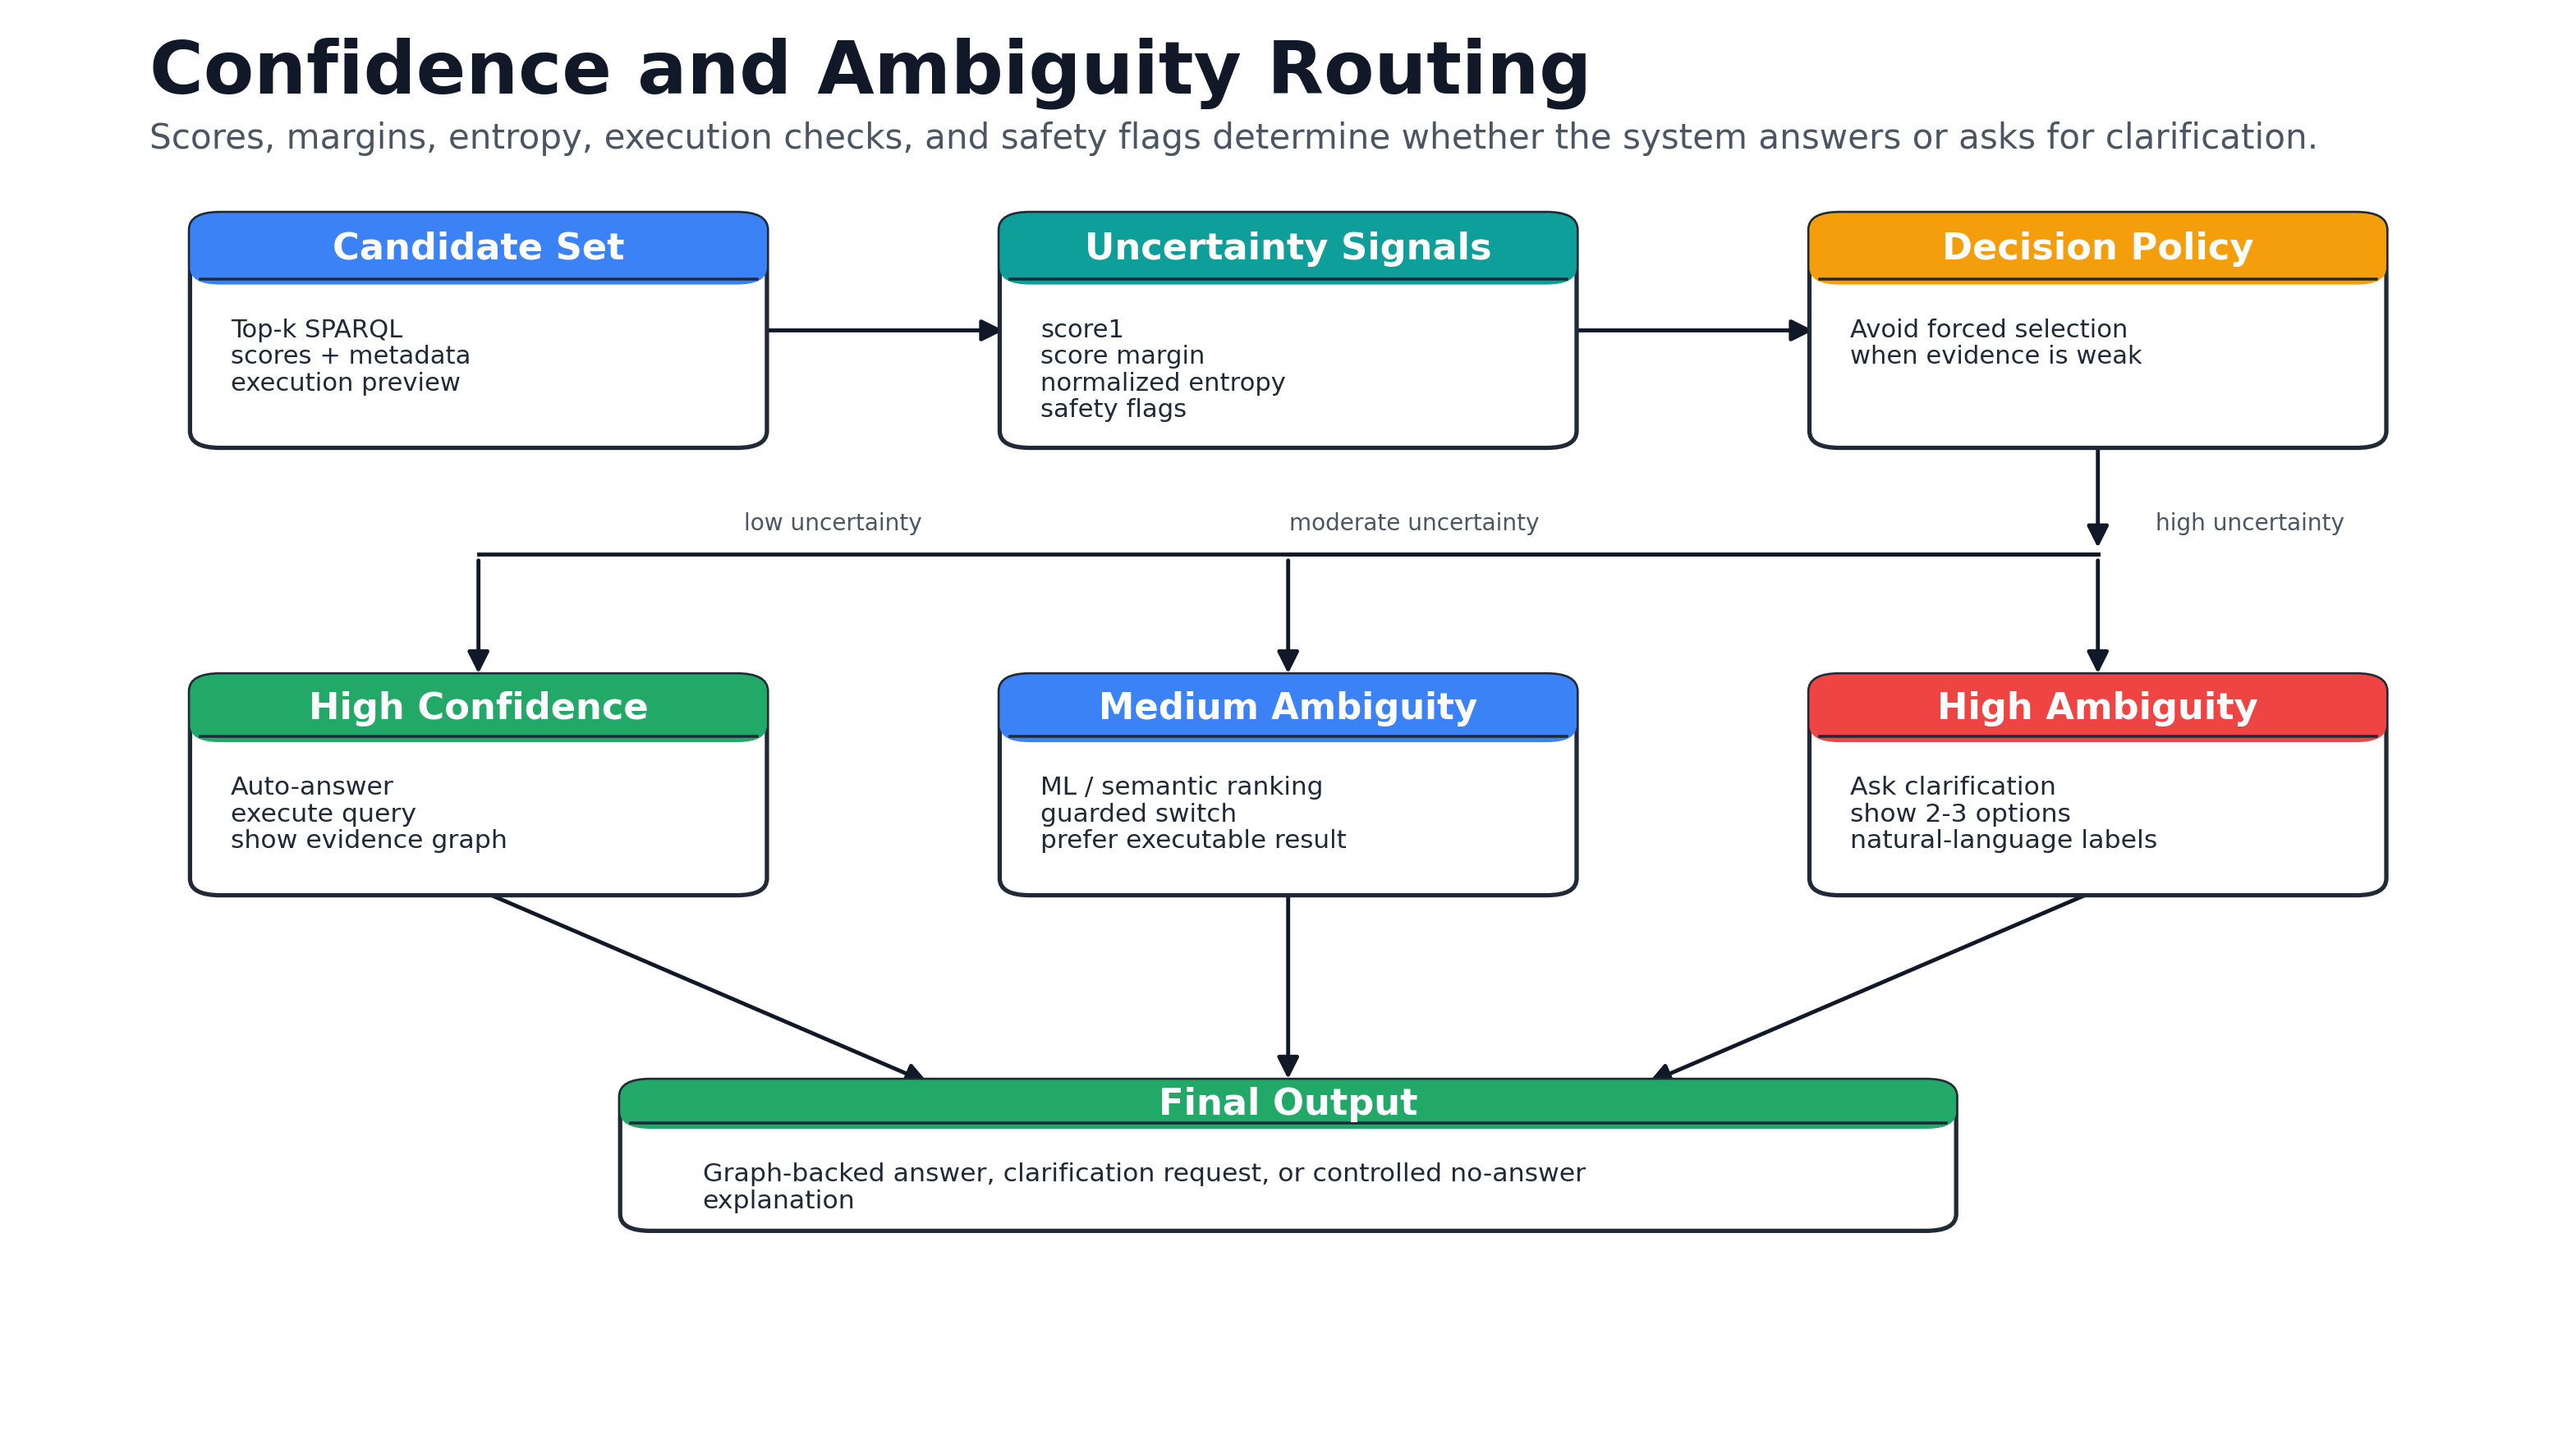
\includegraphics[width=0.92\textwidth]{docs/figures/confidence_ambiguity_routing.png}
\caption{Confidence and ambiguity routing for automatic answers and clarification.}
\label{fig:confidence-ambiguity-routing}
\end{figure}

\begin{table}[ht]
\centering
\caption{Signals used by the confidence and ambiguity router.}
\label{tab:confidence-signals}
\begin{tabular}{p{3.5cm}p{5.5cm}p{4.5cm}}
\hline
\textbf{Signal} & \textbf{Interpretation} & \textbf{Typical action} \\
\hline
High score1 & The selected candidate is strongly preferred by the model & Candidate may be eligible for auto-answer \\
Small margin & Top candidates are close in score & Prefer guarded reranking or clarification \\
High entropy & Candidate probabilities are diffuse & Treat as model uncertainty, inspect alternatives \\
Safety flags & Contract, scope, shape, or capability mismatch detected & Block auto-answer or ask clarification \\
Empty result & Query executes but returns no rows & Penalize candidate or avoid final answer \\
Shape mismatch & Query shape differs from requested answer type & Penalize or clarify \\
\hline
\end{tabular}
\end{table}

Clarification is only useful when it reflects genuine alternative interpretations. The system should not ask for clarification when only one graph-supported interpretation remains. It should also avoid showing unrelated queries merely because they belong to the same broad capability. For example, ``future demand change by region'' should not be clarified against ``how many FutureDemandAnalysis entries exist'' unless the user's question actually contains count intent. Alternative interpretations must differ in capability, dimension, aggregation, or scope in a way that is relevant to the user's question.

\begin{lstlisting}[caption={Confidence-aware decision policy.}, label={lst:confidence-routing-policy}]
if selected_candidate has blocking safety flags:
    ask_clarification_or_show_no_answer()

elif score1 is high and margin is acceptable and query_returns_rows:
    auto_answer()

elif entropy is moderate and candidates are semantically close:
    apply_guarded_ml_and_execution_aware_selection()

else:
    show_natural_language_interpretation_choices(top_candidates)
\end{lstlisting}

The clarification UI presents natural-language interpretations rather than raw SPARQL. Technical SPARQL remains available under an expandable section for debugging and expert users, but the primary choice should be phrased in terms of what the user will see, such as ``average future demand by region'' or ``count companies by shortage status''. This is essential for non-technical users.

\section{Execution and Answer Synthesis}
\label{sec:execution-answer-synthesis}

After a query is selected, it is executed against the True Demand graph. The system supports two execution modes. In the preferred runtime configuration, queries are sent to an Apache Jena Fuseki SPARQL endpoint. Fuseki keeps the graph loaded and indexed, reducing the need to repeatedly parse the full Turtle file. For local or fallback execution, the system can also use RDFLib.

This division allows the prototype to use RDFLib locally while the deployed runtime can rely on a production-like Fuseki endpoint for faster repeated querying.

Execution returns result rows, graph errors, or empty results. These outputs are not treated as a passive final step; they are part of the system's reliability logic. A query that returns no rows should not be presented as a successful high-confidence answer. If the selected candidate fails execution or returns no evidence, the system can inspect lower-ranked candidates, trigger clarification, or show a controlled no-answer response.

\begin{table}[ht]
\centering
\caption{Execution modes supported by the system.}
\label{tab:execution-modes}
\begin{tabular}{p{3.2cm}p{5.2cm}p{5.2cm}}
\hline
\textbf{Mode} & \textbf{Role} & \textbf{Practical implication} \\
\hline
Fuseki endpoint & Executes SPARQL over the loaded True Demand graph & Faster runtime behavior after server startup; suitable for the UI \\
RDFLib local graph & Parses and executes locally from \texttt{graph.ttl} & Useful fallback, but slower for repeated queries \\
Preview execution & Executes candidate queries before final selection in selected modes & Helps avoid empty or shape-inconsistent answers \\
\hline
\end{tabular}
\end{table}

The answer synthesis module converts result rows into natural language. It must respect the answer shape requested by the user. If the query returns grouped rows, the answer should summarize the grouped breakdown rather than converting the result into a highest-value answer unless the user explicitly asked for highest, top, maximum, or minimum. If the result contains a single scalar, the answer can be concise. If the result contains many grouped rows, the answer should report the number of rows and summarize representative groups while preserving access to the raw table or evidence graph in the UI.

\begin{table}[ht]
\centering
\caption{Answer-shape handling during synthesis.}
\label{tab:answer-shape-synthesis}
\begin{tabular}{p{3.4cm}p{5.6cm}p{4.6cm}}
\hline
\textbf{Question type} & \textbf{Expected query/result shape} & \textbf{Answer behavior} \\
\hline
Scalar count & One row with count value & Report the count directly \\
Grouped breakdown & Multiple rows with group variables and metric values & Summarize as grouped results, not as top-one ranking \\
Ranking question & Ordered rows or explicit max/min aggregation & Report highest/lowest result and optionally context \\
List lookup & One column or small table of names/labels & List returned values or summarize count and examples \\
No result & Empty row set & State that no graph-backed answer was found \\
\hline
\end{tabular}
\end{table}

This stage closes the loop between query selection and user-facing answer quality. A correct query can still be presented poorly if answer synthesis ignores the requested shape. Conversely, clear synthesis makes the graph result understandable for non-technical users.

\section{User Interface}
\label{sec:user-interface}

The user interface is implemented as a Streamlit application. Its purpose is not only to collect a question and display an answer, but to expose the system's decision process at the right level of detail. The UI therefore supports natural-language question entry, guided examples, capability-aware suggestions, clarification choices, execution status, answer synthesis, evidence graph visualization, and a confidence-routing dashboard.

The main QA page is designed around a simple workflow. The user enters a question in natural language. If the question matches a direct graph-supported capability, the system answers quickly and displays the result. If the system detects multiple plausible interpretations, it asks the user to choose between natural-language options. Each option can expose additional details and technical SPARQL for debugging, but the default view is business-oriented.

The UI also includes an evidence graph. After execution, the system can show the graph area related to the selected query and result. This helps users understand that the answer is grounded in the knowledge graph rather than generated from free text. For ontology-level exploration, WebVOWL can be used as a separate visualization tool for the schema-level ontology. WebVOWL is useful for understanding classes and relationships, while the Streamlit evidence graph is useful for showing query-specific answer evidence.

\begin{figure}[ht]
\centering
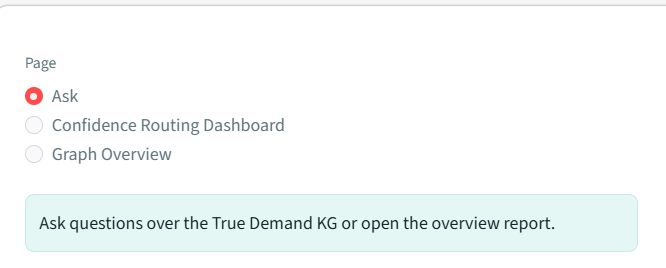
\includegraphics[width=0.98\textwidth]{docs/figures/ui_answer_page.png}
\caption{Streamlit UI answer page showing KG-aware autocomplete, the auto-answer decision, and the answer evidence graph. File: \texttt{docs/figures/ui_answer_page.png}.}
\label{fig:ui-answer-page}
\end{figure}

\begin{figure}[ht]
\centering
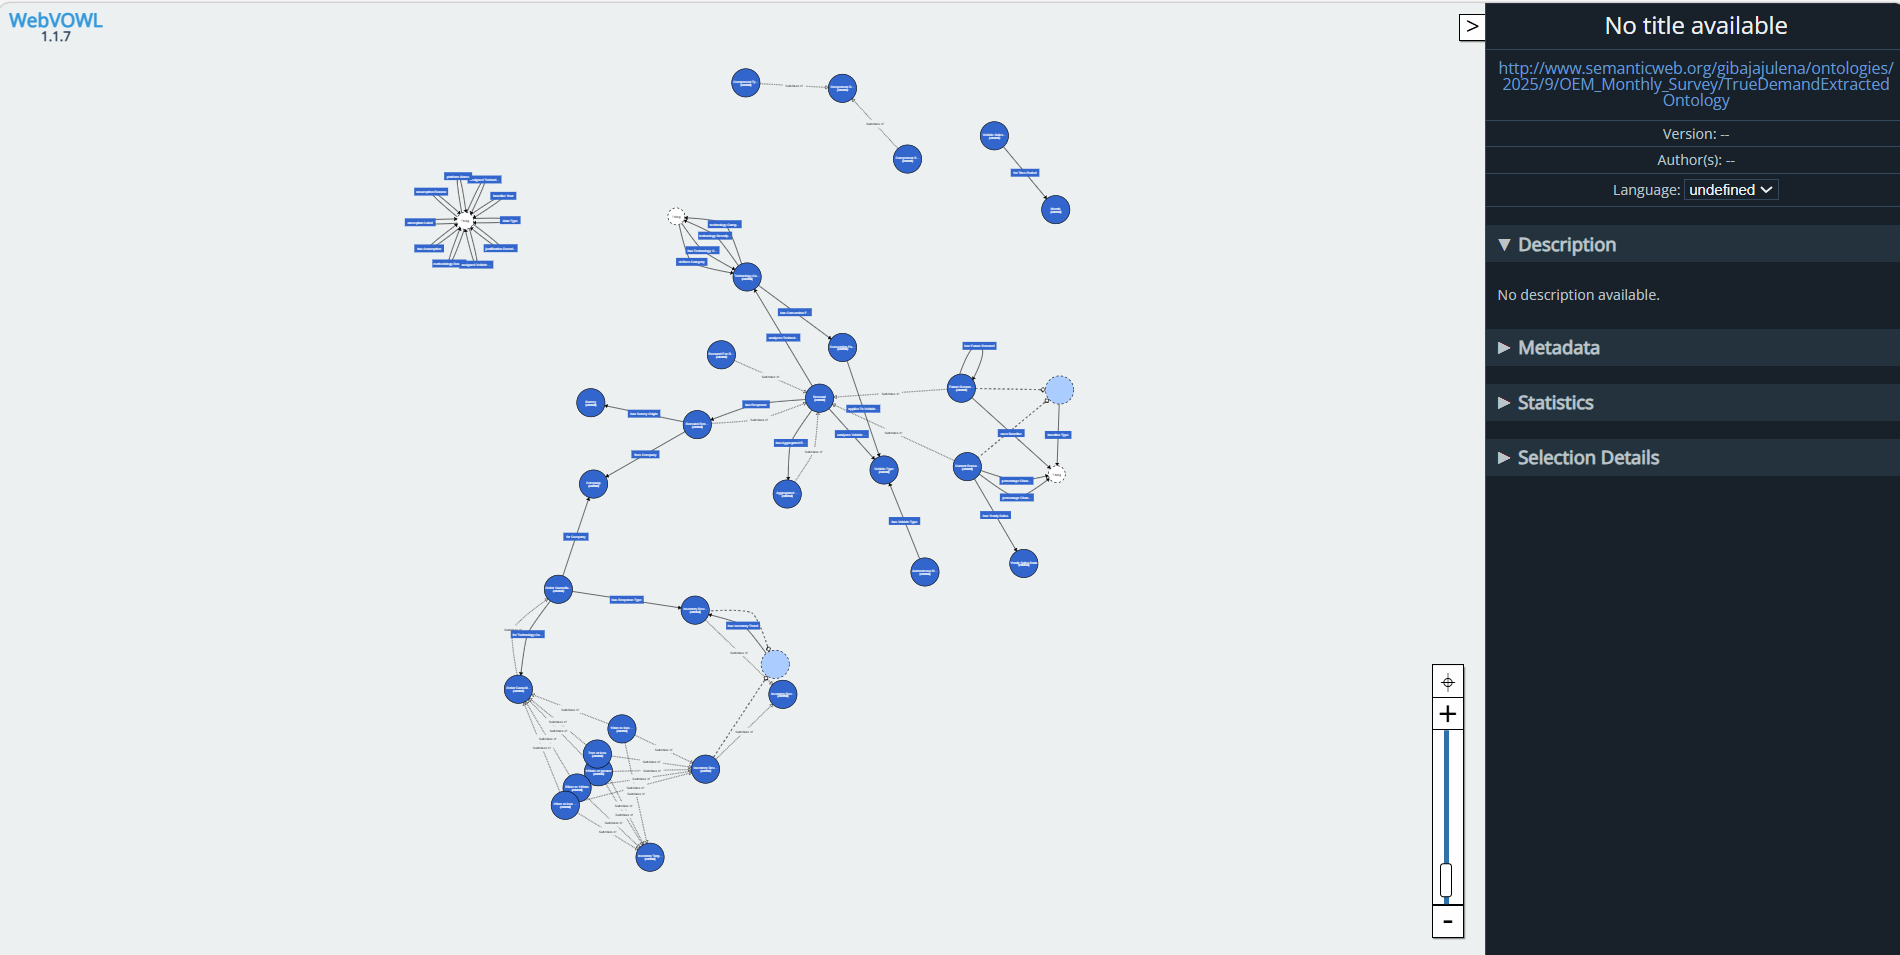
\includegraphics[width=0.98\textwidth]{docs/figures/webvowl_ontology_view.png}
\caption{WebVOWL ontology view for schema-level exploration of the True Demand KG. File: \texttt{docs/figures/webvowl_ontology_view.png}.}
\label{fig:webvowl-ontology-view}
\end{figure}

\begin{table}[ht]
\centering
\caption{Main UI elements and their purpose.}
\label{tab:ui-elements}
\begin{tabular}{p{3.5cm}p{5.8cm}p{4.2cm}}
\hline
\textbf{UI element} & \textbf{Purpose} & \textbf{Target user benefit} \\
\hline
Question input & Allows free natural-language questions & No SPARQL knowledge required \\
Guided examples / builder & Provides graph-supported question patterns & Reduces invalid or unsupported requests \\
Autocomplete / suggestions & Shows graph-aware terms and capabilities & Helps users phrase answerable questions \\
Clarification cards & Shows 2--3 plausible interpretations in natural language & Avoids forced wrong answers \\
Technical SPARQL expander & Shows generated query for expert inspection & Debugging and transparency \\
Answer panel & Presents synthesized graph-backed answer & Business-readable output \\
Evidence graph & Shows entities and relationships used by the answer & Trust and explainability \\
Confidence dashboard & Shows routing metrics and high/low-confidence cases & Evaluation and system diagnosis \\
\hline
\end{tabular}
\end{table}

The UI is intentionally organized so that non-technical users see concise labels first, while technical details remain available when needed. For example, clarification options should be phrased as ``average autonomous-driving development by vehicle type'' rather than as raw query descriptions. The SPARQL query is still available, but it is not the primary decision surface for the user.

From an architecture perspective, the UI is also the place where the ambiguity-aware design becomes visible. The user sees whether the system answered automatically, asked for clarification, or could not find a graph-backed answer. This makes the system more transparent than a black-box LLM response and aligns with the thesis goal of reliable query selection under ambiguity.

\section{Summary}
\label{sec:architecture-summary}

The final system architecture combines deterministic and probabilistic components. Direct graph-supported routing handles frequent answerable questions without LLM calls. The LLM is reserved for cases where candidate generation is needed. Generated candidates are validated, featurized, ranked, and routed through confidence and ambiguity checks. Execution is performed over the full True Demand graph, preferably through Fuseki, and answers are synthesized into natural language with evidence shown in the UI.

The architecture therefore addresses the main weaknesses of a naive LLM-to-SPARQL system. It reduces unnecessary LLM usage, avoids answering unsupported graph paths, separates candidate generation from candidate selection, and gives the user a clarification path when automatic selection would be unreliable.
